\begin{figure}[ht]
    \centering
    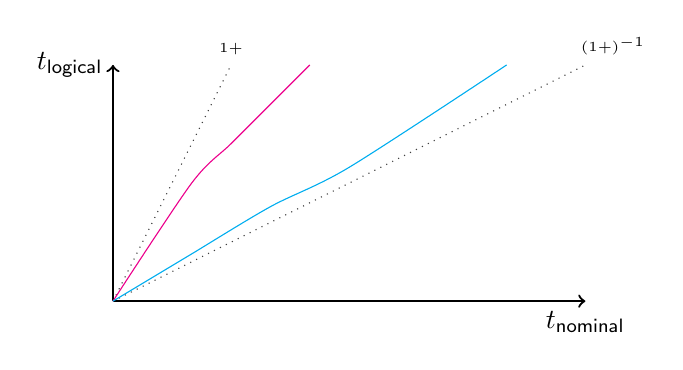
\begin{tikzpicture}
        \draw[->, thick] (0, 0) -- (6, 0) node[below] {$t_{\mathsf{nominal}}$};
        \draw[->, thick] (0, 0) -- (0, 3) node[left] {$t_{\mathsf{logical}}$};

        \draw[dotted, color = darkgray] (0, 0)--(6, 3) node[above, color = black, xshift=1em] {\tiny $(1 + \clockDrift)^{-1}$};
        \draw[dotted, color = darkgray] (0, 0)--(1.5, 3) node[above, color = black] {\tiny $1 + \clockDrift$};

        \draw[opacity=0]  (0,0) -- (1,1) -- (1.5, 2) -- (2, 2.5)  -- (3, 3);

        \draw [magenta] plot [smooth] coordinates { (0,0) (1,1.5) (1.5, 2) (2, 2.5) (2.5, 3)};

        \draw [cyan] plot [smooth] coordinates { (0, 0) (0.5, 0.3) (1, 0.6) (2, 1.2) (3, 1.7) (5, 3)};
    \end{tikzpicture}

    \caption{An illustration of drifting clocks within a $(0.5, 2)$-linear envelope (i.e., $\clockDrift = 1$). Without clock synchronization, two clocks (illustrated in magenta and cyan, respectively) deviate from each other unboundedly.}
    \label{fig:drifting-clocks}
\end{figure}
